\subsection{Negative}
Here negative \st{is not} multiplying by $-1$. It is this transformation:
\[s=L-1-r\]
So sum of image and its negative will be completely white.

\subsubsection{Octave}

\paragraph*{}In MATLAB \texttt{imcomplement} function does the same.
\paragraph*{}http://matlab.izmiran.ru/help/toolbox/images/imcomplement.html says:

\begin{displayquote}
    each pixel value is subtracted from the maximum pixel value supported by the
    class (or 1.0 for double-precision images) and the difference is used as the
    pixel value in the output image.\\
    \dots\\
    If IM is an intensity or RGB image of class \emph{double}, you can use the expression \texttt{1-IM} instead of this function. If IM is a binary image, you can use the expression \texttt{~IM} instead of this function.
\end{displayquote}

\subsubsection{Octave lab}
\begin{Verbatim}[frame=single,label=negative,vspace=0pt]
    > pkg load image; %for calling imhist
    > A=imread("a.png");
    > A=rgb2gray(A); % for doing imhist
    > I=255-A;
    > figure;
    > subplot(2,2,1);imshow(A);
    > subplot(2,2,1);imshow(A);title("A");
    > subplot(2,2,2);imshow(I);title("I");
    > subplot(2,2,3);imhist(A);title("Hist of A");
    > subplot(2,2,4);imhist(I);title("Hist of I");
\end{Verbatim}  
The output is \autoref{fig:negative}. As you can see, histogram
diagram of negative is result of horizontally flipping the histogram of original
image around center of range; which is $\frac{L-1}{2}$. 
\begin{figure}[htb!]
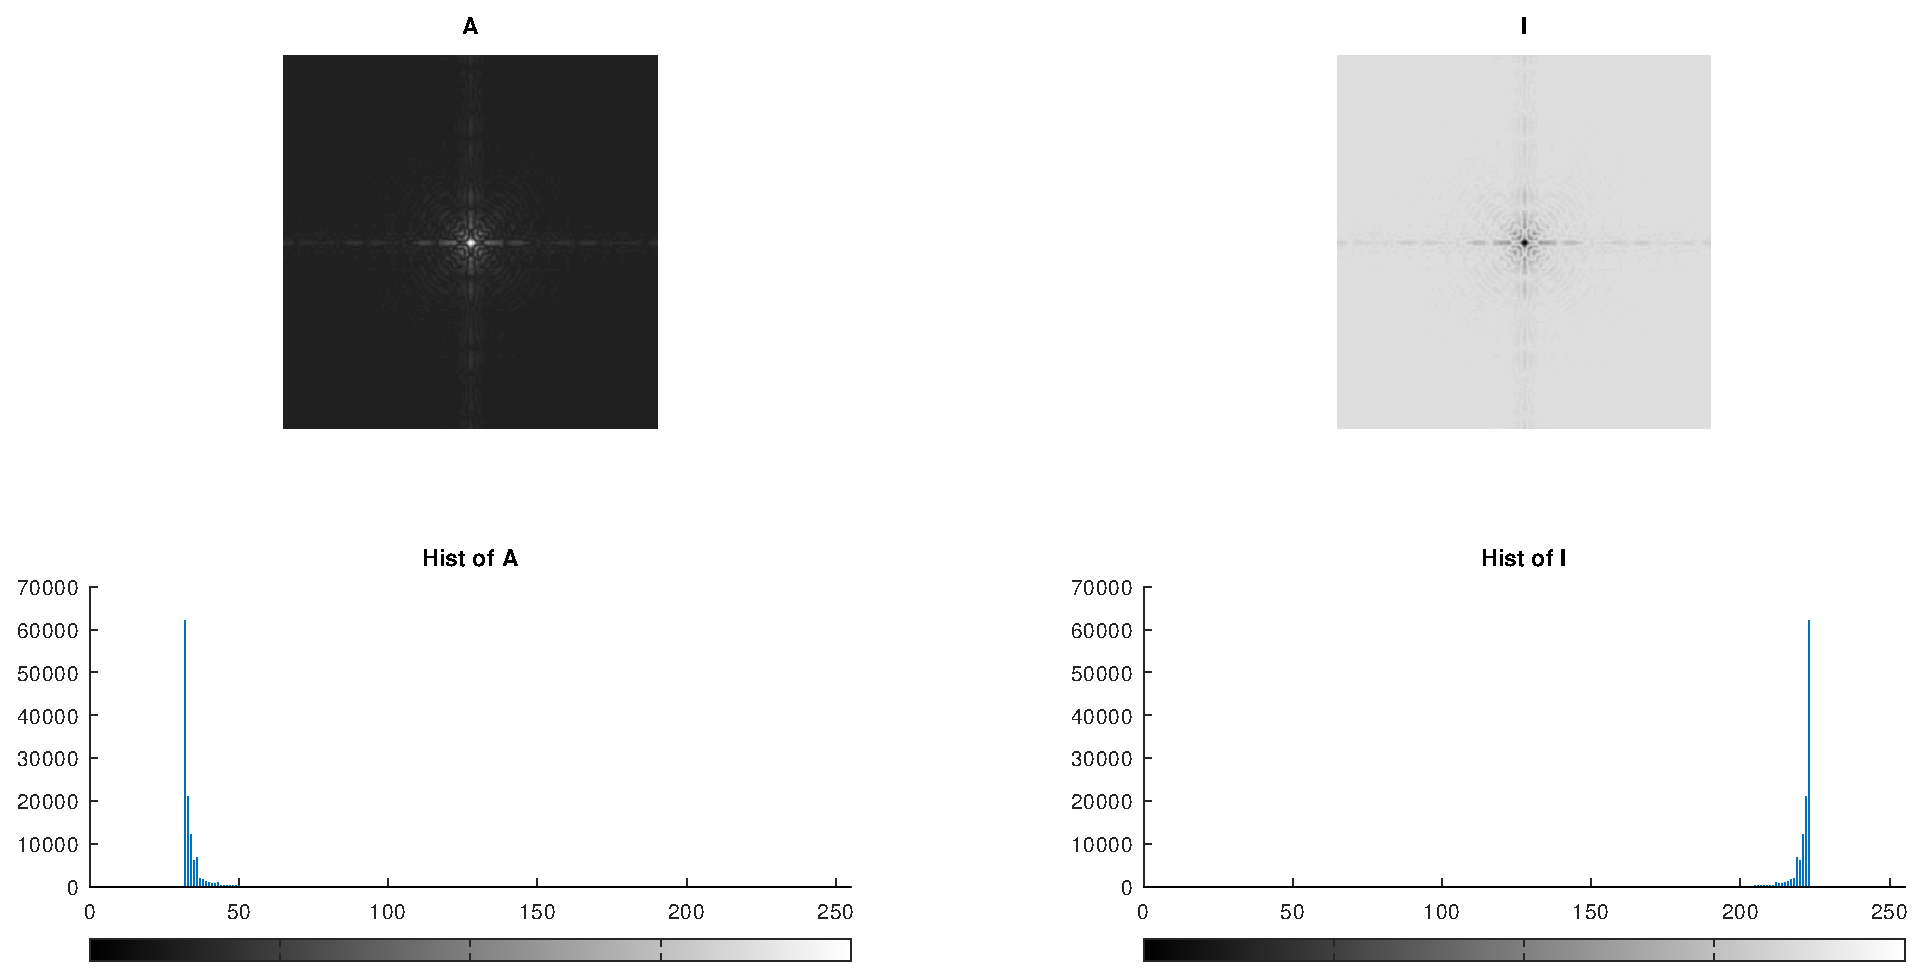
\includegraphics[scale=0.4]{negative.eps}
\centering
\caption{Negative transformation and histogram}
\label{fig:negative}
\end{figure}

\pagebreak
        

        
